\documentclass{article}
\usepackage{amsthm}
\usepackage{amsmath}
\usepackage{graphicx}
\usepackage{tikz}
\usepackage{wasysym}
\usepackage{subcaption}

\newtheorem{problem}{Problem}

\begin{document}
\title{More Graph Algorithms}
\author{Henry Z. Lo}
\maketitle

\section{Transitive Closure}
\begin{problem}
Given a list of train tickets, each of which contain a source and destination airport, construct another graph where an edge between $a$ and $b$ denotes that $b$ is reachable from $a$.
\end{problem}

By reachable, we mean that there is some path from $a$ to $b$.  As an example, suppose we are given the following list:
\begin{center}
\begin{tabular}{l|l}
Source & Destination \\
\hline
San Antonio & Dallas \\
Dallas & San Antonio, Austin \\
Austin & Dallas, Houston \\
Houston & Austin \\
Boston & New York \\
New York & Philadelphia, Boston \\
Philadelphia & Boston \\
\end{tabular}
\end{center}
This is a graph (figure \ref{routes}) in the form of an adjacency list.  We model the problem as an undirected graph, though the solution is similar for directed graphs.  The graph and its transitive closure can be visualized in figure \ref{closure}.

\begin{figure}
\centering
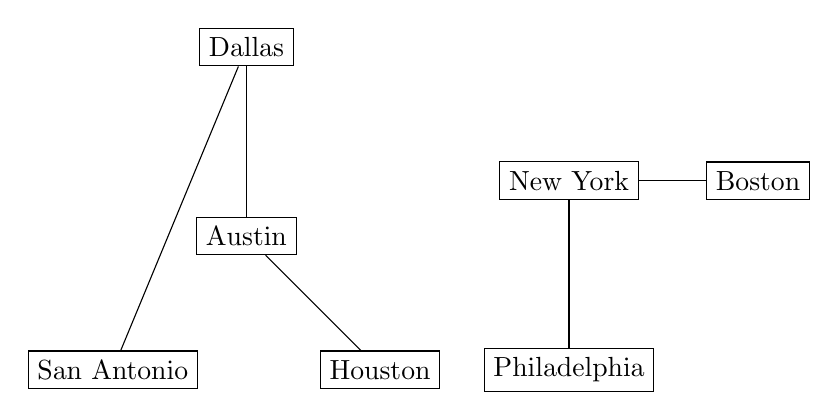
\begin{tikzpicture}[node distance=2.4cm, main node/.style={draw}]
\node[main node]                        (austin)     {Austin};
\node[main node, above of=austin]       (dallas)     {Dallas};
\node[main node, below right of=austin] (houston)    {Houston};
\node[main node, below left of=austin]  (sanantonio) {San Antonio};

\node[main node, right of=houston]      (philly)     {Philadelphia};
\node[main node, above of=philly]       (ny)         {New York};
\node[main node, right of=ny]           (boston)     {Boston};
\path
(austin)     edge node {} (dallas)
             edge node {} (houston)
(dallas)     edge node {} (sanantonio)
(boston)     edge node {} (ny)
(ny)         edge node {} (philly)
;
\end{tikzpicture}
\caption{Undirected graph representing train routes. \label{routes}}
\end{figure}

\begin{figure}
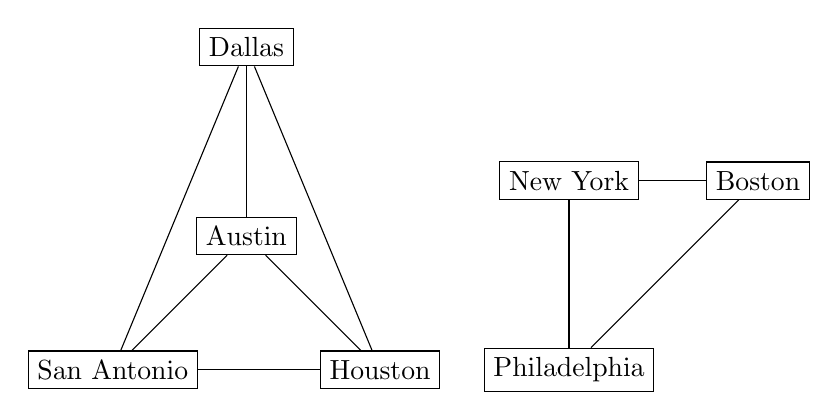
\begin{tikzpicture}[node distance=2.4cm, main node/.style={draw}]
\node[main node]                        (austin)     {Austin};
\node[main node, above of=austin]       (dallas)     {Dallas};
\node[main node, below right of=austin] (houston)    {Houston};
\node[main node, below left of=austin]  (sanantonio) {San Antonio};

\node[main node, right of=houston]      (philly)     {Philadelphia};
\node[main node, above of=philly]       (ny)         {New York};
\node[main node, right of=ny]           (boston)     {Boston};
\path
(austin)     edge node {} (dallas)
             edge node {} (houston)
             edge node {} (sanantonio)
(dallas)     edge node {} (sanantonio)
             edge node {} (houston)
(houston)    edge node {} (sanantonio)
(boston)     edge node {} (ny)
             edge node {} (philly)
(ny)         edge node {} (philly)
;
\end{tikzpicture}
\caption{Transitive closure for figure \ref{routes}. \label{closure}}
\end{figure}

\subsection{Algorithm}
The idea behind the Warshall algorithm is to add edges between nodes reachable by one intermediate node.  Once we do this, another pair of nodes will be reachable by one intermediate node.  By doing this over and over, we can connect all nodes which have paths to each other.

The algorithm:
\begin{verbatim}
  function warshall():
    for k from 1 to V
      for i from 1 to V
        for j from 1 to V
          if edge exists between i,k and edge exists between k,j
            add edge i,j
\end{verbatim}

Why does this work?  In the first iteration of the outer loop, the algorithm connects all nodes which have node 1 as an intermediate node.  Next, it connects all nodes which have node 1 or 2 as intermediate nodes. Eventually, it connects all nodes which have nodes 1 to V as intermediate nodes.

The algorithm here is a triple for loop, so runtime is simply $O(V^3)$.

\subsection{Example}
If we go in the order of the adjacency list, then the Warshall algorithm will do the following in each iteration of the outer loop:
\begin{enumerate}
\item San Antonio is not an intermediate node for any pair, so nothing happens.
\item Dallas is an intermediate between Austin and San Antonio, so we add an edge between them.
\item Due to the last step, Austin bridges San Antonio and Houston, so we add an edge between those two.  Also add an edge between Dallas and Houston.
\item Houston bridges nodes which already have an edge, so we do nothing.
\item Boston does not bridge nodes, so do nothing.
\item New York bridges Boston and Philadelphia, add edge.
\item Philadelphia adds nothing new.
\end{enumerate}
In short, the following edges are added to the graph in figure \ref{routes} in order:
\begin{center}
Austin $\rightarrow$ San Antonio \\
San Antonio $\rightarrow$ Houston \\
Dallas $\rightarrow$ Houston \\
Boston $\rightarrow$ Philadelphia
\end{center}

\section{Topological Sorting}
\begin{problem}
Given a list of classes and their prerequisites, order the classes based on the earliest semester (first, second, third) that you can take them.
\end{problem}

As an example, consider the computer science degree requirements at the UMass Boston:
\begin{center}
\begin{tabular}{l|l}
Course & Prerequisites \\
\hline
CS110 & \\
CS285 & \\
MATH140 & \\
CS240 & CS110 \\
CS210 & CS110 \\
MATH260 & MATH140 \\
CS310 & CS210, CS240 \\
CS320 & CS110, MATH260 \\
CS341 & CS240 \\
CS410 & CS310, CS320 \\
CS420 & CS320 \\
CS444 & CS310, CS341 \\
CS450 & CS310, CS320 \\
CS451 & CS310, CS420 \\
\end{tabular}
\end{center}

We can think of courses as nodes, and a course's prerequisites as directed edges pointing to that course.  Thus, we have a directed acyclic graph (DAG).  

Given this graph, we want to first find the set of nodes which have no dependencies, then the nodes which only have those dependencies.  Putting the nodes in this order gives us a \textit{topological sort}.  This ordering reflects the "levels" in the graph shown in figure \ref{classes}.

\begin{figure}
\centering
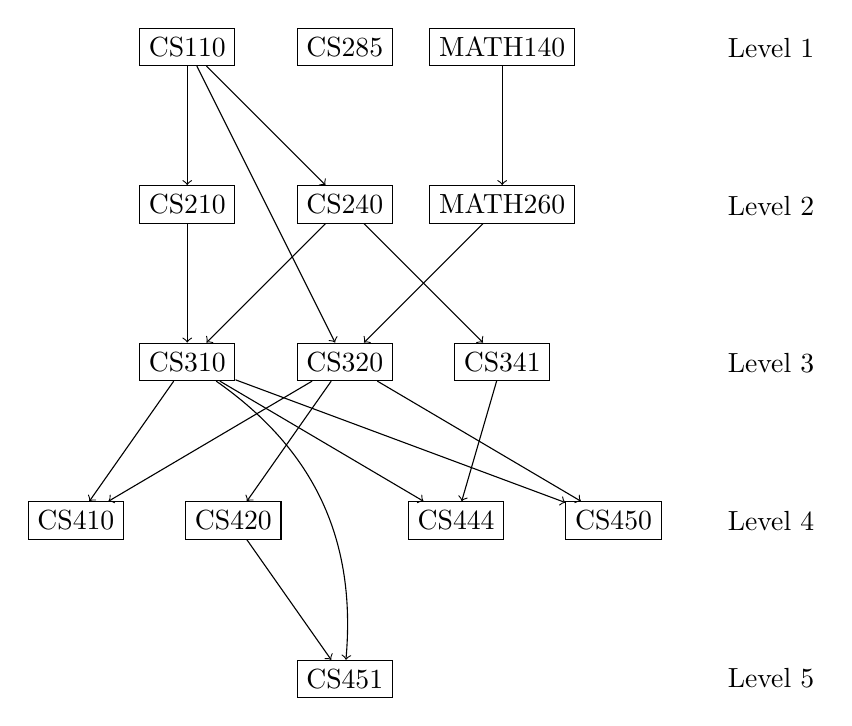
\begin{tikzpicture}[->, node distance=2cm, main node/.style={draw}]
\node[main node]                 (cs110)   {CS110};
\node[main node, right of=cs110] (cs285)   {CS285};
\node[main node, right of=cs285] (math140) {MATH140};
\node[main node, below of=cs110] (cs210)   {CS210};
\node[main node, right of=cs210] (cs240)   {CS240};
\node[main node, right of=cs240] (math260) {MATH260};
\node[main node, below of=cs210] (cs310)   {CS310};
\node[main node, right of=cs310] (cs320)   {CS320};
\node[main node, right of=cs320] (cs341)   {CS341};
\node[main node, below left of=cs320, yshift=-.6cm] (cs420)   {CS420};
\node[main node, left of=cs420] (cs410)   {CS410};
\node[main node, below right of=cs320, yshift=-.6cm] (cs444)   {CS444};
\node[main node, right of=cs444] (cs450)   {CS450};
\node[main node, below right of=cs420, yshift=-.6cm] (cs451)   {CS451};

\node[main node, draw=none, right of=cs450] (lvl4) {Level 4};
\node[main node, draw=none,below of=lvl4]  (lvl5) {Level 5};
\node[main node, draw=none,above of=lvl4]  (lvl3) {Level 3};
\node[main node, draw=none,above of=lvl3]  (lvl2) {Level 2};
\node[main node, draw=none,above of=lvl2]  (lvl1) {Level 1};
\path
(cs110)   edge node {} (cs210)
          edge node {} (cs240)
          edge node {} (cs320)
(math140) edge node {} (math260)
(cs210)   edge node {} (cs310)
(cs240)   edge node {} (cs310)
          edge node {} (cs341)
(math260) edge node {} (cs320)
(cs310) [bend left] edge node {} (cs451)
        [bend left=0]  edge node {} (cs444)
          edge node {} (cs410)
          edge node {} (cs450)
(cs341)   edge node {} (cs444)
(cs320)   edge node {} (cs410)
          edge node {} (cs420)
          edge node {} (cs450)
(cs420)   edge node {} (cs451)
;
\end{tikzpicture}
\caption{Directed acyclic graph representing the class requirements for a computer science major at UMass Boston. \label{classes}}
\end{figure}

\subsection{Algorithm}
The idea behind the algorithm is to first find the nodes without incoming edges.  In a DAG, there is always at least one "ancestor" node.  These ancestor nodes belong to the same "level".  Those nodes which are only dependent on the ancestor nodes form the next level.  The third level of nodes depends only on the first and second level, and so on.  

The key insight is that when we remove the ancestor nodes, the new ancestors are the next topological level.  We can repeatedly find and remove ancestors until we go through all nodes.  If we run out of ancestor nodes without going through all nodes, then there must have been a cycle.

The algorithm for topological sort:
\begin{verbatim}
  function toposort():
    out_q = empty queue
    node_q = queue of nodes with nodes with no parents
    while node_q is not empty
      remove node n1 from node_q
      queue n1 onto out_q
      for each child node n2
        remove edge from n1 to n2
        if n2 has no more parents, add to node_q   
    return out_q   
\end{verbatim}

\subsection{Analysis}
We assume that getting a node's parents or children can be done in constant time.  This is possible if we use two adjacency lists: one to map from the node to its children, and one to map to its parents.  Line 2 then takes $O(V)$ time.

The code within the while loop also runs in $O(V)$ time.

The for loop runs once for each child of the current node.  In total, it runs exactly once for each edge, since iterating through all children of all nodes is equivalent to traversing all edges.  Thus, even though it is within another loop, it must be noted that it runs a $total$ of $O(E)$ times.

In total, this topological sorting algorithm runs in $O(V + E)$, or linear, time.

\subsection{Example}
Going back to the problem of finding the order for classes in figure \ref{classes}, the first few iterations of the topological sorting algorithm will look like this:
\begin{enumerate}
\item Initially, the node queue will contain CS110, CS285, and MATH140.
\item We take out CS110 and its edges, and put CS110 in the output queue.
\item Then we check to see if CS110's children (CS210, CS240, CS240) have any parents left.  CS210 and CS240 do not, so they are put onto the node queue.
\item Then we take out CS285.  It has no edges, so we continue.
\item We take out MATH140 from the node queue.  Its edges are removed, leaving MATH260 without parents.  We put MATH260 onto our topological ordering.
\item Now we have CS210.  We remove its edges.  CS310, its child, still has a parent, so we don't do anything else.
\item We remove CS240 and its nodes.  This orphans CS310 and CS341, which we then put on the queue.
\end{enumerate}
We continue until done.  The resulting topological ordering will look like:
\begin{center}
CS110 $\rightarrow$ CS285 $\rightarrow$ MATH140 $\rightarrow$ CS210 $\rightarrow$ CS240 $\rightarrow$ MATH260 $\rightarrow$ CS310  
$\rightarrow$ CS320 $\rightarrow$ CS341 $\rightarrow$ CS410 $\rightarrow$ CS420 $\rightarrow$ CS444 $\rightarrow$ CS450 $\rightarrow$ CS451
\end{center}

\section{Longest Path}
\begin{problem}
Given a set of tasks, their completion times, and their dependencies on other tasks, compute the total time it takes to finish all tasks. \end{problem}

We can model this type of task set with a PERT chart (see figure \ref{pert}), a graphical model which contains tasks as nodes, and dependencies as edges.  Edge weights represent the time it takes to complete the parent task.  

\begin{figure}
\centering
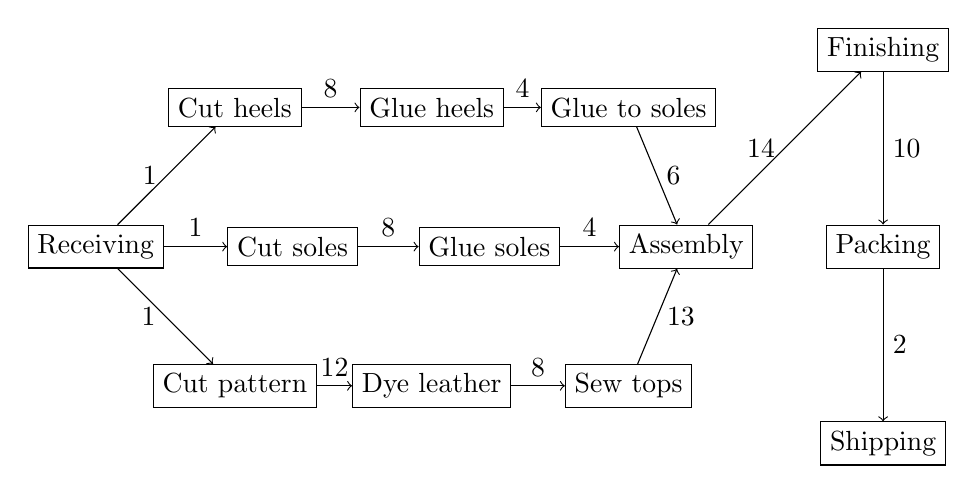
\begin{tikzpicture}[->, node distance=2.5cm, main node/.style={draw}]
\node[main node]                   (1)  {Receiving};
\node[main node, above right of=1] (2)  {Cut heels};
\node[main node, right of=1]       (3)  {Cut soles};
\node[main node, below right of=1] (4)  {Cut pattern};
\node[main node, right of=2]       (5)  {Glue heels};
\node[main node, right of=3]       (6)  {Glue soles};
\node[main node, right of=4]       (7)  {Dye leather};
\node[main node, right of=5]       (8)  {Glue to soles};
\node[main node, right of=7]       (9)  {Sew tops};
\node[main node, right of=6]       (10) {Assembly};
\node[main node, right of=10]      (12) {Packing};
\node[main node, above of=12]      (11) {Finishing};
\node[main node, below of=12]      (13) {Shipping};

\path
(1)   edge node [left]  {1}  (2)
      edge node [above] {1}  (3)
      edge node [left]  {1}  (4)
(2)   edge node [above] {8}  (5)
(3)   edge node [above] {8}  (6)
(4)   edge node [above] {12} (7)
(5)   edge node [above] {4}  (8)
(6)   edge node [above] {4}  (10)
(7)   edge node [above] {8}  (9)
(8)   edge node [right] {6}  (10)
(9)   edge node [right] {13} (10)
(10)  edge node [left]  {14} (11)
(11)  edge node [right] {10} (12)
(12)  edge node [right] {2}  (13)
;
\end{tikzpicture}
\caption{PERT chart for shoe construction workflow.  Edge weights represent days needed for the given task. \label{pert}}
\end{figure}

In PERT charts we are interested in the critical path, the longest path in the graph.  This path in figure \ref{pert} is:
\begin{center}
Receiving $\rightarrow$ Cut pattern $\rightarrow$ Dye leather $\rightarrow$ Sew tops $\rightarrow$ Assembly $\rightarrow$ Finishing $\rightarrow$ Packing $\rightarrow$ Shipping
\end{center}
The critical path here has a length of 60 days, which is the time it takes to complete all tasks.

\subsection{Longest path problem}
In general, the longest path problem is easy to compute, but not fast.  The obvious solution is to use a breadth-first or depth-first search.

These traversal algorithms run in linear time for finding a certain node, because we only visit each node exactly once.  We do not traverse edges already traversed.

However, here we are looking for a \textit{path}.  Even though we should not encounter a node twice in the same path, we can encounter the node multiple times in different paths.  This makes the corresponding \textit{path} tree much larger than the BFS/DFS tree.  

See figure \ref{path-tree} for an example.  Note that to solve the longest path problem, we actually need to initialize the path from every single node.  The number of possible paths grows factorially with the number of nodes.  Hence, unlike the $O(V)$ BFS/DFS tree, the path tree is $O(V!)$.

\begin{figure}
\centering
\begin{subfigure}{.5\textwidth}
\centering
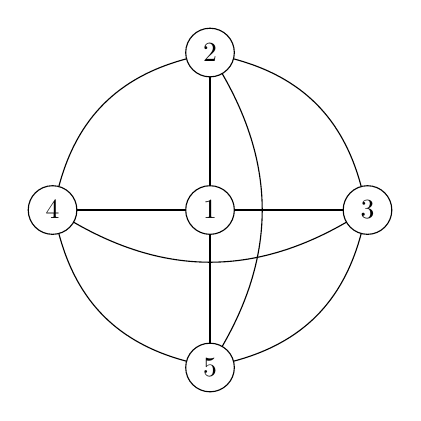
\begin{tikzpicture}[node distance=2cm, main node/.style={draw,circle}]
\node[main node]             (1)  {1};
\node[main node, above of=1] (2)  {2};
\node[main node, right of=1] (3)  {3};
\node[main node, left of=1]  (4)  {4};
\node[main node, below of=1] (5)  {5};

\path
(1) edge node {} (2)
    edge node {} (3)
    edge node {} (4)
    edge node {} (5)
(2) [bend left]  edge node {} (3)
    [bend right] edge node {} (4)
    [bend left]  edge node {} (5)
(3) edge node {} (4)
    edge node {} (5)
(4) [bend right] edge node {} (5)
;
\end{tikzpicture}
\caption{Arbitrary undirected graph. \label{graph}}
\end{subfigure}

\begin{subfigure}{.7\textwidth}
\centering
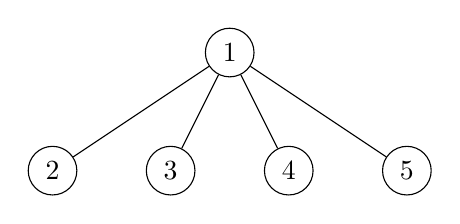
\begin{tikzpicture}[node distance=2cm, main node/.style={draw,circle}]
\node[main node] {1}
 child{node [main node] {2}}
 child{node [main node] {3}}
 child{node [main node] {4}}
 child{node [main node] {5}}
;
\end{tikzpicture}
\caption{BFS tree for this graph, starting from 1. \label{dfstree}}
\end{subfigure}
\begin{subfigure}{1\textwidth}
\centering
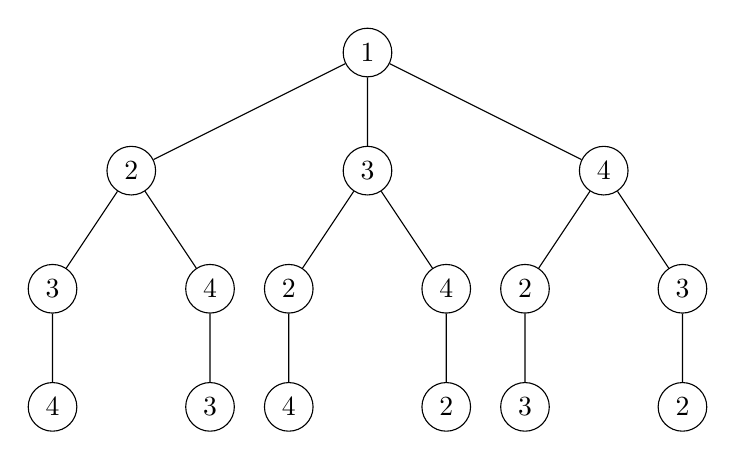
\begin{tikzpicture}[level 1/.style={sibling distance=3cm},
level 2/.style={sibling distance=2cm}, 
level 3/.style={sibling distance=1cm}, main node/.style={draw,circle}]
\node[main node] {1}
 child{node [main node] {2}
  child{node [main node] {3}
   child{node [main node] {4}}}
  child{node [main node] {4}
   child{node [main node] {3}}}}
 child{node [main node] {3}
  child{node [main node] {2}
   child{node [main node] {4}}}
  child{node [main node] {4}
   child{node [main node] {2}}}}
 child{node [main node] {4}
  child{node [main node] {2}
   child{node [main node] {3}}}
  child{node [main node] {3}
   child{node [main node] {2}}}}
   ;
\end{tikzpicture}
\caption{Path tree, starting from 1. \label{path}}
\end{subfigure}
\caption{BFS and path tree for a complete graph, starting at node 1. \label{path-tree}}
\end{figure}

There is actually no known solution for finding the longest path in a general graph which is reasonably fast (in polynomial time).  We will discuss this in the next set of notes.  However, for directed acyclic graphs, there is an extremely efficient algorithm. 

\subsection{Longest path in a DAG}
Despite the general difficulty of finding the longest path, we can see very quickly in figure \ref{pert} that there are only 3 paths to consider:
\begin{itemize}
\item receiving $\rightarrow$ cut pattern $\rightarrow$ \ldots $\rightarrow$ shipping
\item receiving $\rightarrow$ cut heels $\rightarrow$ \ldots $\rightarrow$ shipping
\item receiving $\rightarrow$ cut soles $\rightarrow$ \ldots $\rightarrow$ shipping.
\end{itemize}

We only consider these three because we know that any longest path must start at a parentless node and end at a childless node.  If it didn't, then we can always make a longer path by including a parent or child.  

For example, cut soles $\rightarrow$ \ldots $\rightarrow$ packing could not possibly be a longest path, because we can add receiving to the front of this path, and shipping to the end to make it longer.

This suggests that we can use topological ordering to help find the longest path.

\subsection{Algorithm}
The idea behind finding the longest path in a DAG is first topologically sort all nodes, then iterate through this list.  For each node, only consider the \textit{longest} path from the ancestor nodes, and use that as its current value.  Note that if we perform computations in this order, by the time we process a node, we have already processed its parents.

The algorithm:
\begin{verbatim}
  function longestDAGpath():
    q = toposort(nodes)
    m = map from nodes to integer
    for node in q
      if node has no parents
        m[node] = 0
      else
        for each parent p of node
          m[node] = max(m[node], m[p] + edge value of p->node)
    len = infinity
    for n in set of childless nodes
      len = min(len, m[n])
    return len
\end{verbatim}

Compare this with Dijkstra's algorithm.

Topological sorting, as mentioned, takes $O(V+E)$.  Just as in topological sorting, the outer loop in this algorithm occurs $O(V)$ times, and the inner loop occurs exactly $O(E)$ times in total.  Finding childless nodes and iterating through them is also $O(V)$.  Hence, the entire algorithm is linear, $O(V+E)$.

\subsection{Example}

In the PERT chart example, \texttt{m} changes as follows:
\begin{enumerate}
\item $\texttt{m[receiving]}=0$
\item $\texttt{m[cut heels]}=1$
\item $\texttt{m[cut soles]}=1$
\item $\texttt{m[cut pattern]}=1$
\item $\texttt{m[glue heels]}=8+1=9$
\item $\texttt{m[glue soles]}=8+1=9$
\item $\texttt{m[dye leather]}=12+1=13$
\item $\texttt{m[glue to soles]}=4+9=13$
\item $\texttt{m[sew tops]}=8+13=21$
\item $\texttt{m[assembly]}=max(13+6, 9+4, 21+13)=34$
\end{enumerate}
After step 10, everything else is pretty linear.  Note that we only consider the longest path to get to assembly.  Everything after assembly uses this time.  Thus, by the time we get to shipping, we will be using the longest path length to get to shipping, which was through the cut patterns route.
\end{document}
